\section{Introduction}
\label{sec:introduction}

% state the learning objective 

\hspace{0,5cm} This report is being made for the subject of Circuit Theory and Electronics Fundamentals and is related to the $1^{st}$ laboratory.

The objective of this laboratory assignment is to study a circuit containing 7 resistors, 1 voltage source, 1 current source, 1 current controlled voltage source and 1 voltage controlled current source.

The display of this circuit can be seen in Figure~\ref{fig:circuito}.

In Section~\ref{sec:analysis} we will analise theorically the circuit and present the results obtained by Octave.

Secondly, in Section~\ref{sec:simulation} we will simulate the circuit using ngspice, present the results obtained and compare them with the ones gathered from Section~\ref{sec:analysis}.

The conclusions of this study are outlined in Section~\ref{sec:conclusion}.

\begin{figure}[h] \centering
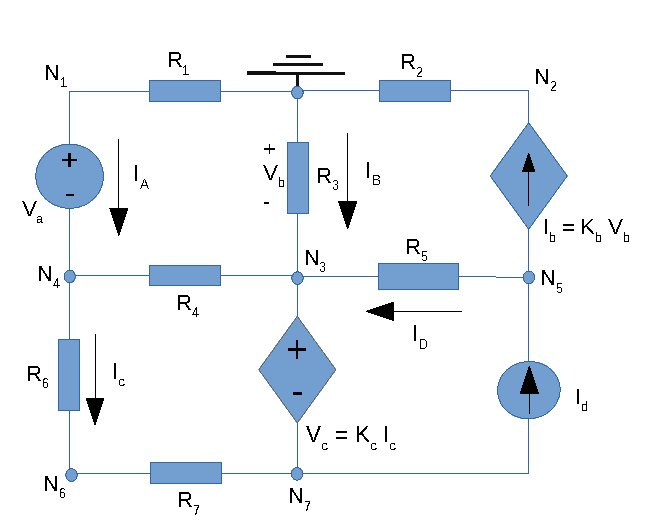
\includegraphics[width=0.7\linewidth]{circuito.pdf}
\caption{Circuit with the nodes} %mudar legendaaaaaaaaaaa!!!!!!
\label{fig:circuito}
\end{figure}


\begin{center}
Where:

$R_1 = 1.03431507833 $

$R_2 = 2.02853090731$
 
$R3 = 3.1462050633 $

$R_4 = 4.03438547455$ 

$R_5 = 3.12170042214 $

$R_6 = 2.07116379646 $

$R_7 = 1.01597753093 $

$V_a = 5.156959346 $

$I_d = 1.01455683569 $

$K_b = 7.1497941196 $

$K_c = 8.12593642585 $
\end{center}

Units for the values: $V, mA, k\Omega$ and $mS$



